% !Mode:: "TeX:UTF-8"

\chapter{Servlet 项目}

\section{项目需求}

本项目要求使用VUE+Servlet+AJAX技术,开发前后端分离的饿了么Web应用程序。主要设计参照 “饿了么官网网页版”制作,并且仅关注点餐业务线功能,“饿了么官网”中的其它功能暂不涉及。

本项目需要完成的功能大致分为十一个页面:~\\

\subsection{首页功能}
\subsubsection*{\normalsize主要功能}
显示点餐分类信息
\subsubsection*{\normalsize动作}
1.点击点餐分类小图片,跳转到商家列表页面

2.点击下方菜单栏中的“订单”,跳转到历史订单页面~\\

\subsection{商家列表页面功能}
\subsubsection*{\normalsize主要功能}
1.根据点餐分类显示商家列表信息

2.如果处于登录状态,那些需要查询购物车中是否有此商家的食品。如果有,在页面上显示食品数量
\subsubsection*{\normalsize动作}
点击某个商家,跳转到此商家的详细信息页面~\\

\subsection{商家详细信息页面功能}
\subsubsection*{\normalsize主要功能}
显示商家详细信息及所属食品信息,并自动计算总价
\subsubsection*{\normalsize动作}
1.点击某食品的 + 按钮,食品数量加 1

2.点击某食品的 - 按钮,食品数量减 1

3.点击“去结算”按钮,跳转到确认订单页面

4.如果没有登录,那么上述三个动作会自动跳转到登录页面~\\

\subsection{确认订单页面功能}
\subsubsection*{\normalsize主要功能}
1.确认订单信息是否正确

2.选择送货地址
\subsubsection*{\normalsize动作}
1.点击送货地址,跳转到送货地址列表页面

2.点击“去支付”按钮,跳转到支付页面~\\

\subsection{在线支付页面功能}
\subsubsection*{\normalsize主要功能}
显示订单信息及订单明细信息
\subsubsection*{\normalsize动作}
无(点餐业务流程到此结束)~\\

\subsection{送货地址列表页面功能}
\subsubsection*{\normalsize主要功能}
显示当前用户的送货地址信息
\subsubsection*{\normalsize动作}
1.点击某个送货地址,跳转回确认订单页面

2.点击“新增”按钮,跳转到新增送货地址页面

3.点击“编辑”按钮,跳转到送货地址编辑页面

4.点击“删除”按钮,删除此送货地址~\\

\subsection{新增送货地址页面功能}
\subsubsection*{\normalsize主要功能}
添加新的送货地址
\subsubsection*{\normalsize动作}
点击“保存”按钮,添加新的送货地址,并跳转到送货地址列表页面~\\

\subsection{编辑送货地址页面功能}
\subsubsection*{\normalsize主要功能}
编辑送货地址
\subsubsection*{\normalsize动作}
点击“更新”按钮,保存编辑后的送货地址,并跳转到送货地址列表页面~\\

\subsection{登录页面功能}
\subsubsection*{\normalsize主要功能}
用户登录
\subsubsection*{\normalsize动作}
1、 点击“登陆”按钮,进行登陆业务处理。如果登陆成功,跳转到上一个页面

2、 点击“去注册”按钮,跳转到注册页面~\\

\subsection{注册页面功能}
\subsubsection*{\normalsize主要功能}
注册新用户
\subsubsection*{\normalsize动作}
点击“注册”按钮,进行新用户注册。注册成功后,跳转到登陆页面~\\

\subsection{历史订单页面功能}
\subsubsection*{\normalsize主要功能}
显示用户历史订单信息
\subsubsection*{\normalsize动作}
点击某个历史订单,可以对订单明细信息进行显示和隐藏

\begin{figure}[H]
    \centering
    \subfigure{
        \begin{minipage}[t]{0.22\linewidth}
            \centering
            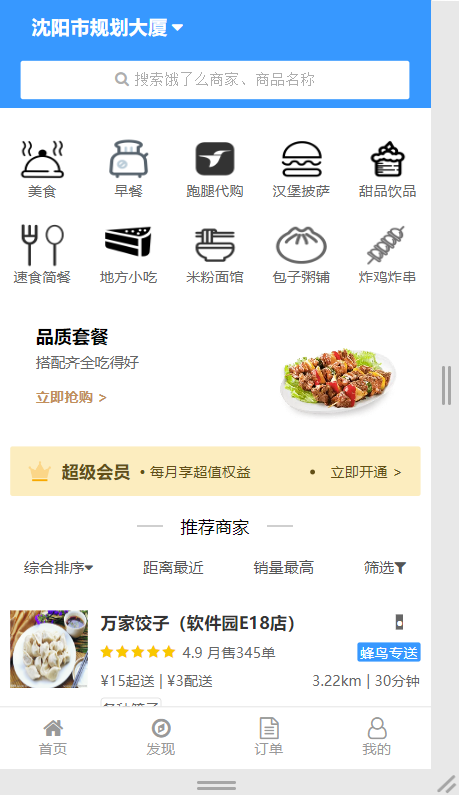
\includegraphics[width=3.2cm,height=6.4cm]{figures/3.1.1.png}\\
            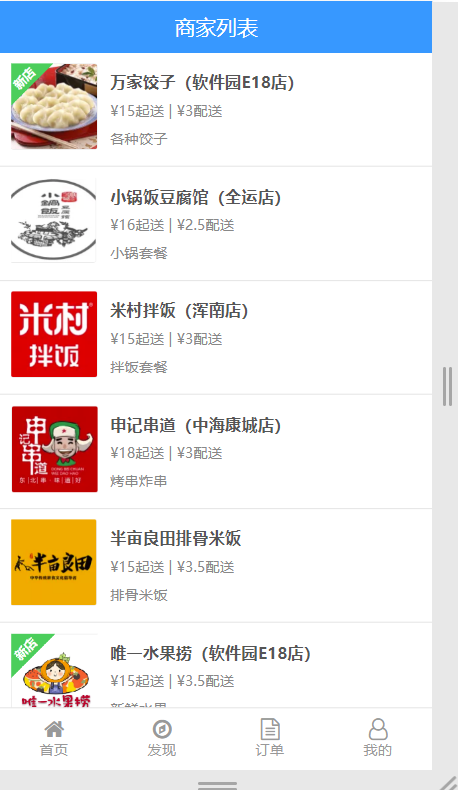
\includegraphics[width=3.2cm,height=6.4cm]{figures/3.1.2.png}\\
            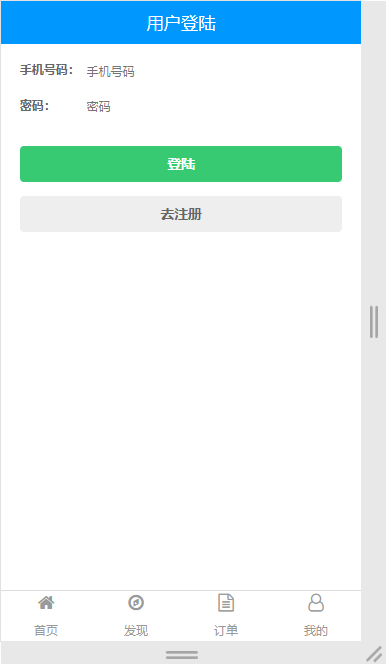
\includegraphics[width=3.2cm,height=6.4cm]{figures/3.1.9.png}\\
        \end{minipage}
    }
    \subfigure{
        \begin{minipage}[t]{0.22\linewidth}
            \centering
            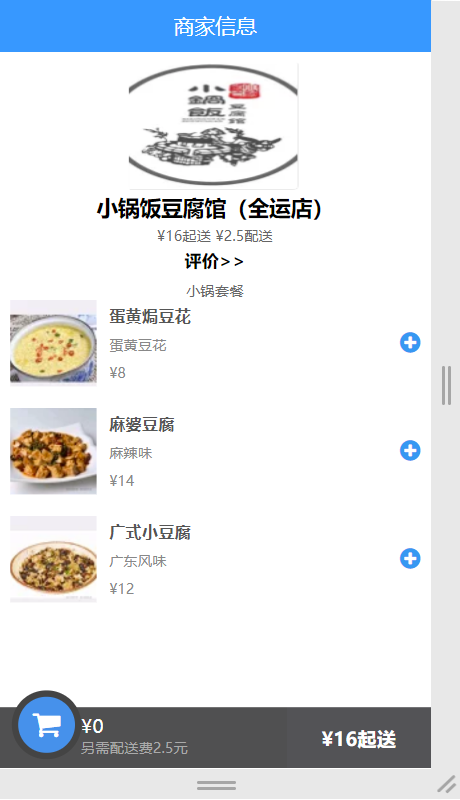
\includegraphics[width=3.2cm,height=6.4cm]{figures/3.1.3.png}\\
            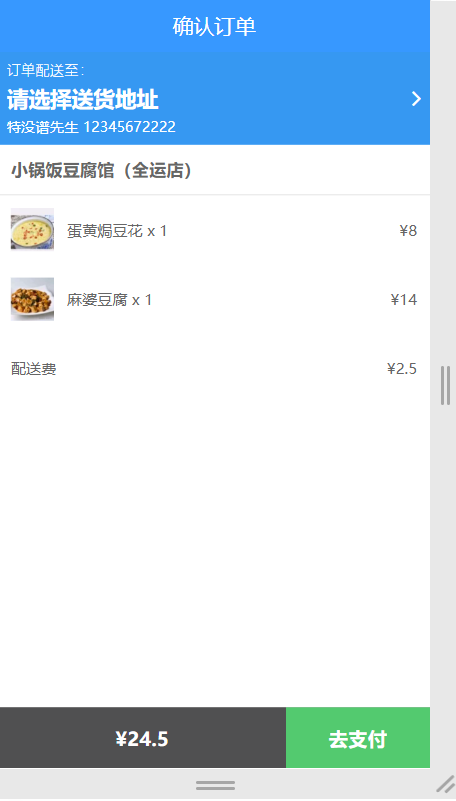
\includegraphics[width=3.2cm,height=6.4cm]{figures/3.1.4.png}\\
            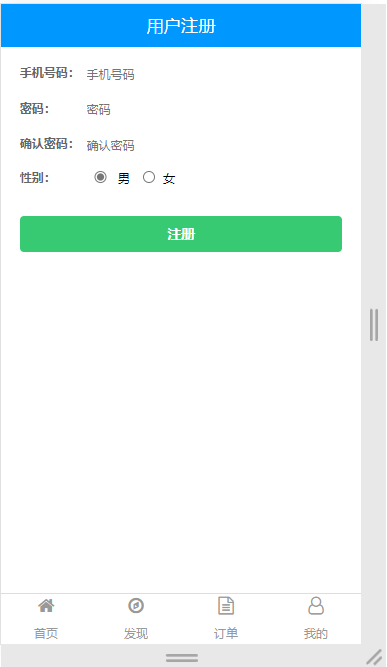
\includegraphics[width=3.2cm,height=6.4cm]{figures/3.1.10.png}\\
        \end{minipage}
    }
    \subfigure{
        \begin{minipage}[t]{0.22\linewidth}
            \centering
            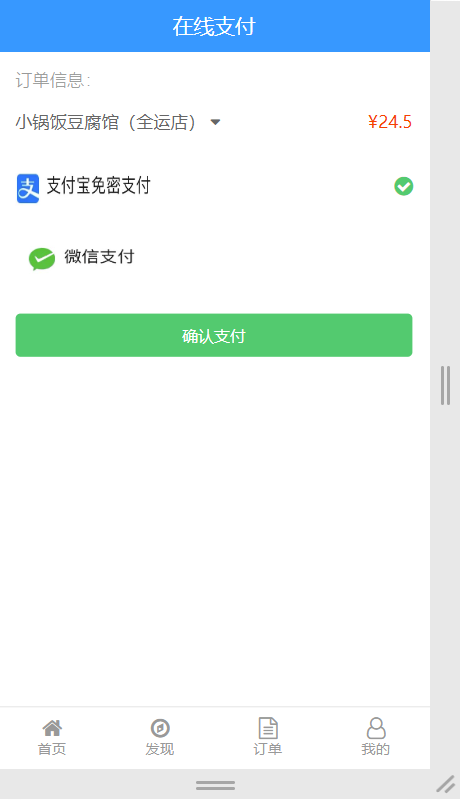
\includegraphics[width=3.2cm,height=6.4cm]{figures/3.1.5.png}\\
            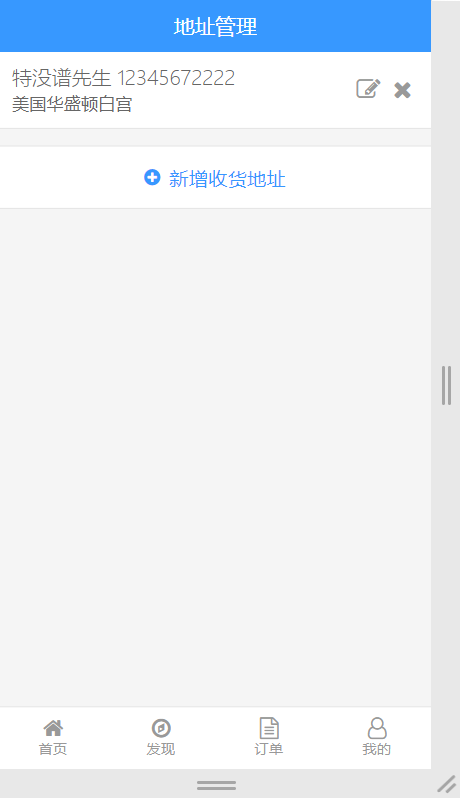
\includegraphics[width=3.2cm,height=6.4cm]{figures/3.1.6.png}\\
            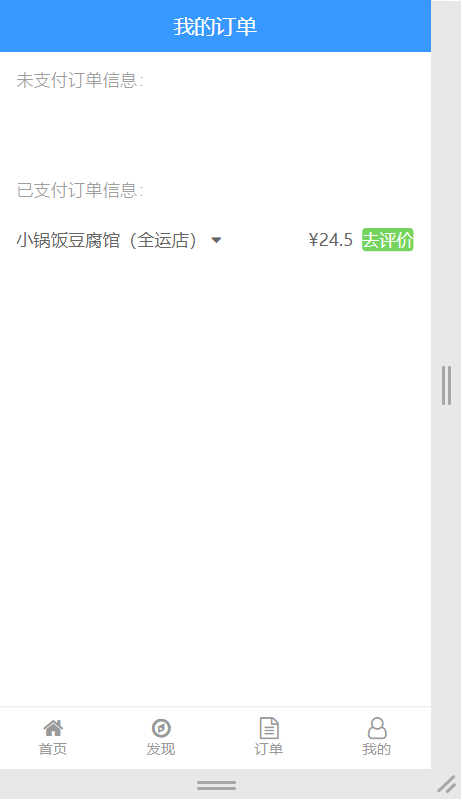
\includegraphics[width=3.2cm,height=6.4cm]{figures/3.1.11.png}\\
        \end{minipage}
    }
    \subfigure{
        \begin{minipage}[t]{0.22\linewidth}
            \centering
            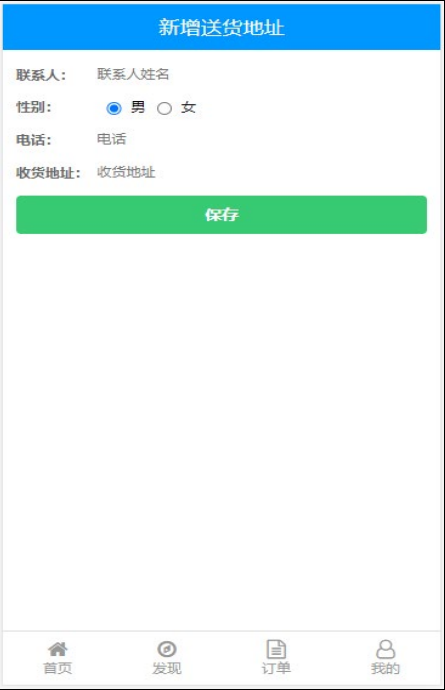
\includegraphics[width=3.2cm,height=6.4cm]{figures/3.1.7.png}\\
            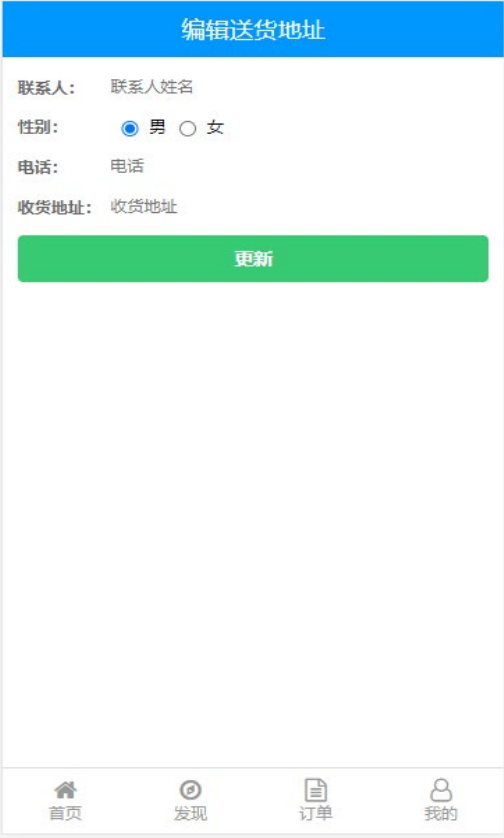
\includegraphics[width=3.2cm,height=6.4cm]{figures/3.1.8.png}\\
        \end{minipage}
    }
    \centering
    \caption{VUE前端页面实现结果}
\end{figure}

\section{项目设计}

\subsection{VUE前端设计}
首先安装cnpm和VueCli开发环境,使用VSCode工具进行项目开发。

接着搭建VueCli模板工程、添加依赖及配置文件。添加font-awesome与axios依赖。
添加图片到src的assets中。
在src目录下添加common.js文件,用于添加一些公用方法。
在工程根目录下添加vue.config.js文件,用于配置前端的端口号。
添加main.js文件,用于判断每个页面是否需要登录才可以使用。
添加App.vue文件,里面设置全局的共通样式。

最后实现各个组件:主页、商家列表、商家详细信息、订单、支付、添加修改用户地址、历史订单、登录、注册和底部导航栏共同组件。~\\

\subsection{数据库设计}
本项目使用MySQL数据库,选择DataGrip作为开发工具。在数据表的设计上,需要创建商家表、食品表、购物车表、送货地址表、订单表、订单明细表、用户表共七张表。

\begin{figure}[H]
    \centering
    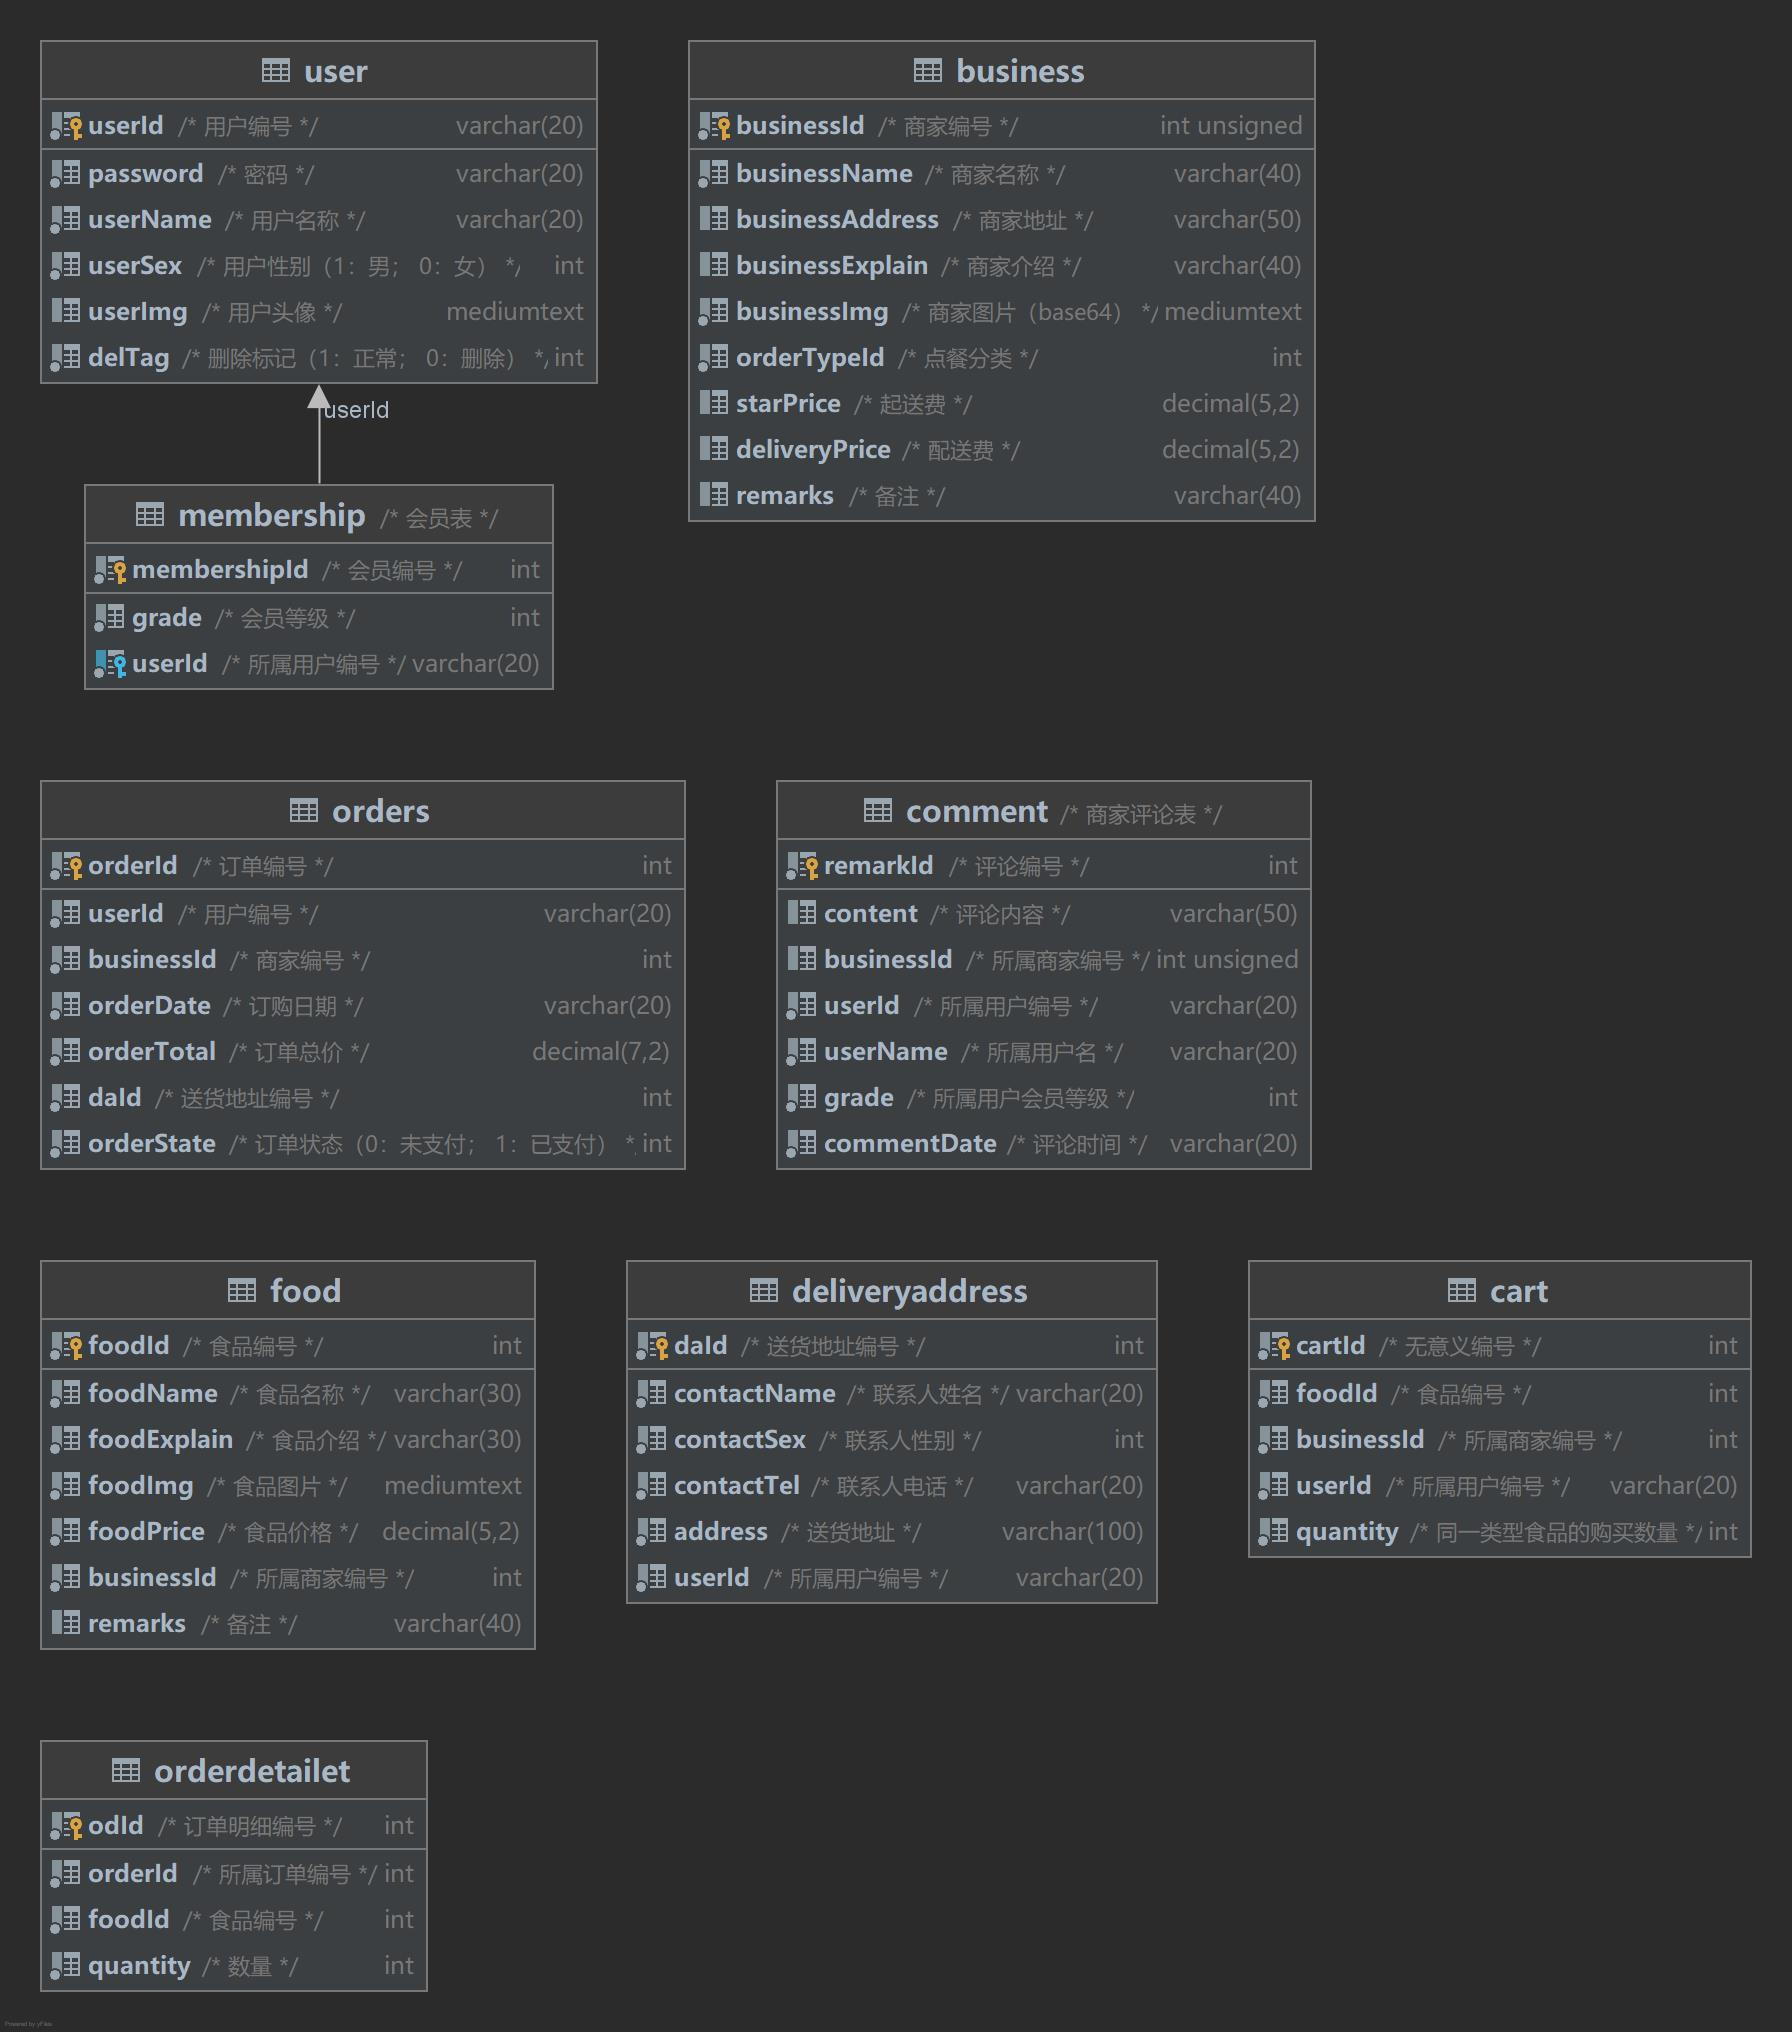
\includegraphics[width=15cm,height=12cm]{figures/table2.jpg}
    \caption{Servlet项目数据表}
\end{figure}

\subsection{Servlet后端设计}

\noindent
一. 开发环境

1. 开发工具:IDEA、DataGrip

2. 检查IDEA的jdk配置:jdk8

3. 检查IDEA的tomcat配置:tomcat 9.0.65

4. 检查IDEA的文件编码配置:utf-8

5. 检查MySQL配置:MySQL 8.0.30~\\

\noindent
二. 开发技术

本项目为JavaWeb项目,在后端使用Servlet技术,Tomcat作为容器进行项目开发。在JavaWeb工程的搭建方面,本项目使用基于Servlet的简易MVC架构,能够很好地解决后端与前端地交互。在响应前端请求方面,使用Jackson将java对象或集合转换为json对象或数组后,返回前端。

\begin{figure}[H]
    \centering
    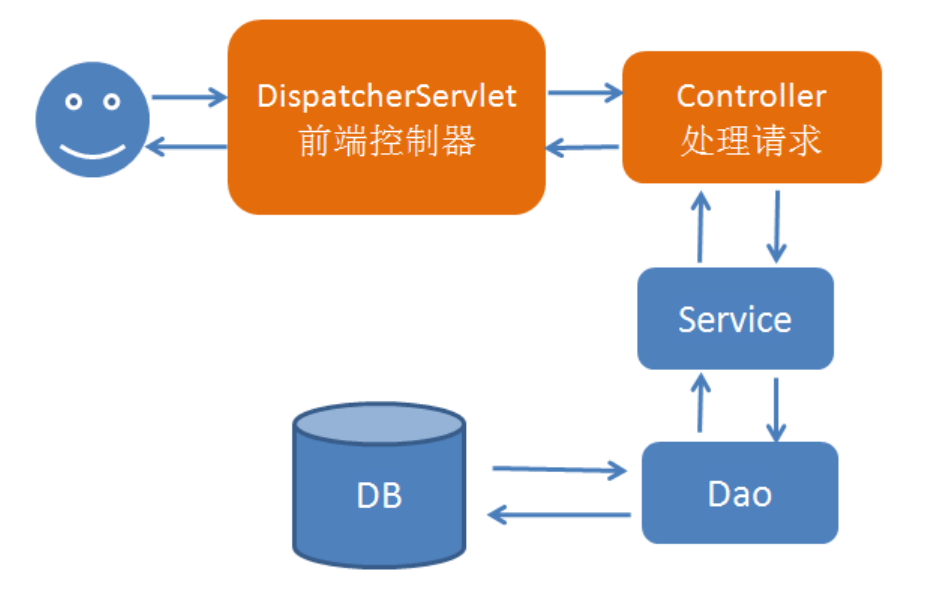
\includegraphics[width=15cm,height=10cm]{figures/MVC.png}
    \caption{Servlet简易MVC架构}
\end{figure}

\noindent
三. 跨域问题解决

本项目使用CORS解决前后端分离开发模式时的跨域问题,它允许浏览器向跨源服务器,发出XMLHttpRequest请求,从而克服了AJAX只能同源使用的限制。实现CORS通信的关键是服务器,只要服务器实现了CORS接口,就可以跨源通信。~\\

\noindent
四. 事务处理解决

本项目将事务的处理放在Service层:

1.Connection的创建与销毁要放在service层。

2.为了保证在同一次请求处理的线程中,service层和dao层都共用同一个Connection对象,需要将Connection对象放入ThreadLocal中。service层和dao层使用的Connection对象一律从ThreadLocal获取。

3.dao层不再处理异常,dao层产生的异常将直接抛给service层进行处理。

4.dao层负责关闭PreparedStatement和ResultSet,service层负责关闭Connection。

\begin{figure}[H]
    \centering
    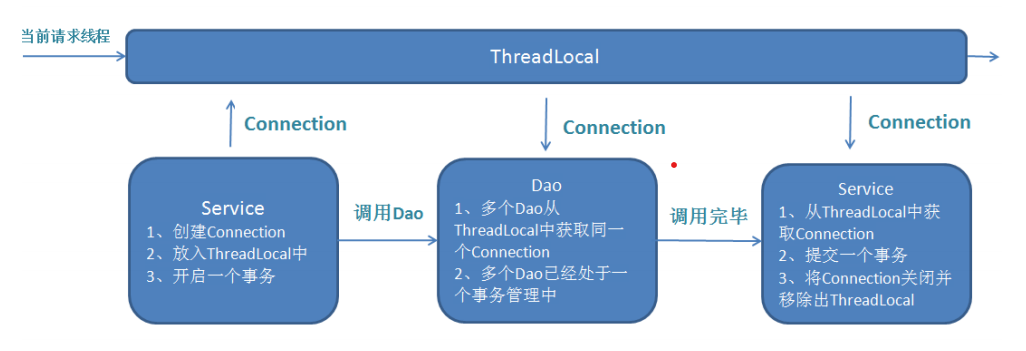
\includegraphics[width=15cm,height=6cm]{figures/thread.png}
    \caption{线程池}
\end{figure}

\noindent
五. 项目结构

本项目主要结构由上到下分为Controller层、Service层、Dao层三层架构:Controller层主要负责与客户端进行交互,接收并响应前端请求;Service层主要负责处理需要实现的业务逻辑;Dao层主要负责对于数据库的操作。

其他软件包主要存放一些功能性代码,framework包主要搭建DispatcherServlet前端控制器,filter包主要解决跨域问题,po包主要存放业务流中所需的持久对象,与数据表相对应,util包中存放一些常用的工具类。

\begin{figure}[H]
    \centering
    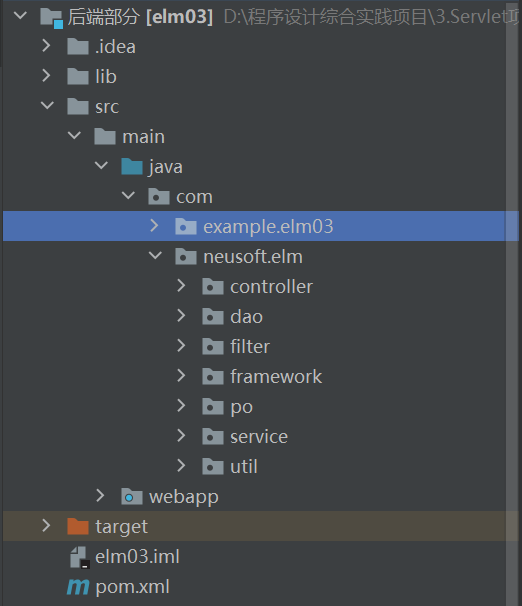
\includegraphics[width=15cm,height=18cm]{figures/structure3.png}
    \caption{项目结构}
\end{figure}

\noindent
六. 服务器接口API

1. Business

1.1 BusinessController/listBusinessByOrderTypeId 

参数:orderTypeId 

返回值:business数组

功能:根据点餐分类编号查询所属商家信息

1.2 BusinessController/getBusinessById 

参数:businessId 

返回值:business对象

功能:根据商家编号查询商家信息~\\

2. Food

2.1 FoodController/listFoodByBusinessId 

参数:businessId 

返回值:food数组

功能:根据商家编号查询所属食品信息~\\

3. Cart

3.1 CartController/listCart 
参数:userId、businessId(可选)

返回值:cart数组(多对一:所属商家信息、所属食品信息)

功能:根据用户编号查询此用户所有购物车信息

\qquad\quad根据用户编号和商家编号,查询此用户购物车中某个商家的所有购物车信息

3.2 CartController/saveCart 

参数:userId、businessId、foodId 

返回值:int(影响的行数)

功能:向购物车表中添加一条记录

3.3 CartController/updateCart 

参数:userId、businessId、foodId、quantity

返回值:int(影响的行数)

功能:根据用户编号、商家编号、食品编号更新数量

3.4 CartController/removeCart 

参数:userId、businessId、foodId(可选)

返回值:int(影响的行数)

功能:根据用户编号、商家编号、食品编号删除购物车表中的一条食品记录

\qquad\quad根据用户编号、商家编号删除购物车表中的多条条记录~\\

4. DeliveryAddress

4.1 DeliveryAddressController/listDeliveryAddressByUserId 

参数:userId 

返回值:deliveryAddress数组

功能:根据用户编号查询所属送货地址

4.2 DeliveryAddressController/getDeliveryAddressById 

参数:daId 

返回值:deliveryAddress对象

功能:根据送货地址编号查询送货地址

4.3 DeliveryAddressController/saveDeliveryAddress 

参数:contactName、contactSex、contactTel、address、userId 

返回值:int(影响的行数)

功能:向送货地址表中添加一条记录

4.4 DeliveryAddressController/updateDeliveryAddress

参数:daId、contactName、contactSex、contactTel、address、userId

返回值:int(影响的行数)

功能:根据送货地址编号更新送货地址信息

4.5 DeliveryAddressController/removeDeliveryAddress 

参数:daId 

返回值:int(影响的行数)

功能:根据送货地址编号删除一条记录~\\

5. Orders

5.1 OrdersController/createOrders 

参数:userId、businessId、daId、orderTotal 

返回值:int(订单编号)

功能:根据用户编号、商家编号、订单总金额、送货地址编号向订单表中添加一条记录,

\qquad\quad并获取自动生成的订单编号,

\qquad\quad然后根据用户编号、商家编号从购物车表中查询所有数据,批量添加到订单明细表中,

\qquad\quad然后根据用户编号、商家编号删除购物车表中的数据。

5.2 OrdersController/getOrdersById 

参数:orderId 

返回值:orders对象(包括多对一:商家信息; 一对多:订单明细信息)

功能:根据订单编号查询订单信息,包括所属商家信息,和此订单的所有订单明细信息

5.3 OrdersController/listOrdersByUserId 

参数:userId 

返回值:orders数组(包括多对一:商家信息; 一对多:订单明细信息)

功能:根据用户编号查询此用户的所有订单信息~\\

6. User

6.1 UserController/getUserByIdByPass 

参数:userId、password 

返回值:user对象

功能:根据用户编号与密码查询用户信息

6.2 UserController/getUserById 

参数:userId 

返回值:int(返回行数)

功能:根据用户编号查询用户表返回的行数

6.3 UserController/saveUser 

参数:userId、password、userName、userSex

返回值:int(影响的行数)

功能:向用户表中添加一条记录~\\

\noindent
七. 业务流程

\begin{figure}[H]
    \centering
    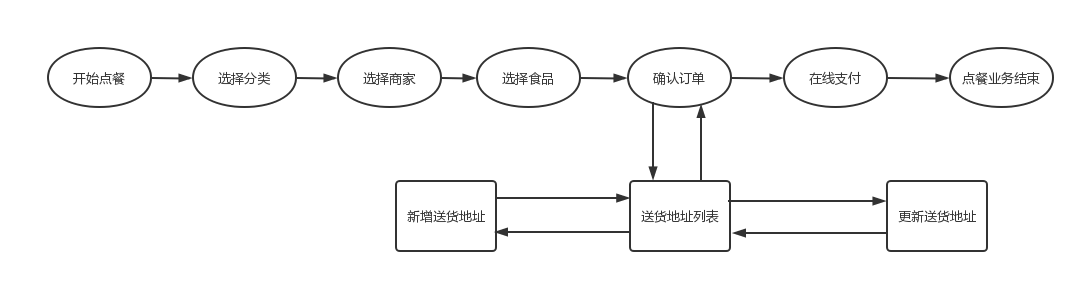
\includegraphics[scale=0.45]{figures/flowchart.png}
    \caption{业务流程图}
\end{figure}

